\documentclass{article}

% if you need to pass options to natbib, use, e.g.:
% \PassOptionsToPackage{numbers, compress}{natbib}
% before loading nips_2016
%
% to avoid loading the natbib package, add option nonatbib:
% \usepackage[nonatbib]{nips_2016}

% \usepackage{nips_2016}

% to compile a camera-ready version, add the [final] option, e.g.:
\usepackage[final]{nips_2016}

\usepackage[utf8]{inputenc} % allow utf-8 input
\usepackage[T1]{fontenc}    % use 8-bit T1 fonts
\usepackage{hyperref}       % hyperlinks
\usepackage{url}            % simple URL typesetting
\usepackage{booktabs}       % professional-quality tables
\usepackage{amsfonts}       % blackboard math symbols
\usepackage{nicefrac}       % compact symbols for 1/2, etc.
\usepackage{microtype}      % microtypography
\usepackage[utf8]{inputenc}
\usepackage{booktabs,floatrow}
\usepackage{graphicx}
\usepackage{color}
\usepackage[font=small]{caption}
%\usepackage{caption}
\usepackage{subcaption}
\usepackage[bottom]{footmisc}

%10-707 Deep Learning Project Final Report\\
\title{Text Classification with Different Neural Networks Approaches}

% The \author macro works with any number of authors. There are two
% commands used to separate the names and addresses of multiple
% authors: \And and \AND.
%
% Using \And between authors leaves it to LaTeX to determine where to
% break the lines. Using \AND forces a line break at that point. So,
% if LaTeX puts 3 of 4 authors names on the first line, and the last
% on the second line, try using \AND instead of \And before the third
% author name.


\author{
  Lindi Chen \\
  Electrical and Computer Engineering\\
  \texttt{lindc@andrew.cmu.edu}\\
  \And
  Yao Mu \\
  Computer Science Department\\
  \texttt{ymu1@andrew.cmu.edu}\\
  \And
  Zhuoqun Chen\\
  Computer Science Department\\
  \texttt{zhuoqunc@andrew.cmu.edu} \\
  %% examples of more authors
  %% \And
  %% Coauthor \\
  %% Affiliation \\
  %% Address \\
  %% \texttt{email} \\
  %% \AND
  %% Coauthor \\
  %% Affiliation \\
  %% Address \\
  %% \texttt{email} \\
  %% \And
  %% Coauthor \\
  %% Affiliation \\
  %% Address \\
  %% \texttt{email} \\
  %% \And
  %% Coauthor \\
  %% Affiliation \\
  %% Address \\
  %% \texttt{email} \\
}

\begin{document}
% \nipsfinalcopy is no longer used

\maketitle

\begin{abstract}
Text classification is the fundamental task for many natural language processing applications. In this paper, we study the text classification problem using different deep learning approaches.  We compare and analyze the performance of different text classification approaches, such as Support Vector Machine (SVM), Convolutional Neural Network (CNN) and Recurrent Neural Network (RNN), etc.
\end{abstract}


%Conventionally, text classification problem is usually addressed using manually-designed feature engineering and feature selection. Deep neural networks  

\section{Introduction}
Text classification has always been the classic topic in natural language processing. Specifically, the task of text classification is to assign pre-defined categories to text documents with high accuracy. Text classification is the building block for a variety of applications, such as web searching, information retrieval, and sentiment analysis. Therefore it has attracted a great deal of research interests.

% Text classification is an essential component in many applications, such as web searching, information filtering, and sentiment analysis. Text classification is gaining its importance in recent years thanks to the explosion of social media, e-commerce, Instant message, and the digitalization of  publication. It has various applications that has huge commercial value. Classification of web pages and news stories could be help to automatically recommend content to the customers. Huge amount of manpower could be saved  in identifying the right category of Emails and feedbacks. With the increasing volume of text published each year, it has become more and more impossible for human beings to perform such task. 

The key issue in text classification lies in feature representation. Several feature representation schema such as word frequency, MI, pLSA, LDA have been introduced to represent discriminative features. However, these methods ignore the contextual information and word sequence. To deal with this issue, Recurrent Neural Networks have been introduced. RNN depends heavily on the construction of its textual tree, and the construction exhibits $O(n^2)$ time complexity. Convolutional neural network in contrast exhibits the ability to extract features and relatively less parameters to train due to parameter sharing. Therefore in this project, we would compare the performance of the above mentioned methods in text classification tasks in detail.

\section{Related Work}
In this section, different machine learning approaches to deal with text classification are surveyed in detail. 

\subsection{Support Vector Machine}

Support Vector Machine [5] models are often used as baseline in text classification task.  An SVM is a kind of large-margin classifier, which is a vector space based machine learning method where the goal is to find a decision boundary between two classes that is maximally far from any point in the training data. Being a 2-class classifier, SVM could also be extended as multi-class classifier as is introduced in [5].  The authors of [4] argue that a SVM with a simple but novel Naive Bayes variant and simple bag of features model are still strong performers on snippet sentiment classification tasks.


\subsection{Convolutional neural network}
Convolutional Neural Networks [6] is often considered as a powerful tool for computer vision, because images intrinsically  have  because of the compositional structure of an image. However, texts are also compositional for many languages. Characters combine to form n-grams, stems, words, phrase, sentences etc [14]. 

Convolutional Neural Networks is applied to Natural Language Processing by learning word vector representations through neural language models.utilize layers with convolving filters that are applied to local features. The pre-trained vectors are based on unsupervised neural language models and publicly available. They are `universal' feature extractors that can be utilized for various text classification tasks.

Most techniques of text classification are based on words, where simple ordered word combinations (e.g. n-grams) and word embeddings (see section section 2.3 and 2.4) are utilized. There are also efforts on exploring character-level features in language processing [1], which applies one-dimensional temporal  convolutional neural networks for text classification.

\subsection{Word2vec Embedding}
Word2vec [7] is a group of related models that are used to produce word embeddings. These models are shallow, two-layer neural networks that are trained to reconstruct linguistic contexts of words. Word2vec takes as its input a large corpus of text and produces a vector space, typically of several hundred dimensions, with each unique word in the corpus being assigned a corresponding vector in the space. Word vectors are positioned in the vector space such that words that share common contexts in the corpus are located in close proximity to one another in the space.

\subsection{GloVe Embedding}
GloVe [8] is an unsupervised learning algorithm for obtaining vector representations for words. Training is performed on aggregated global word-word co-occurrence statistics from a corpus. GloVe is a new global log-bilinear regression model using global matrix factorization and local context window methods. It  efficiently leverages statistical information by training only on the nonzero elements in a word-word co-occurrence matrix, rather than on the entire sparse matrix or on individual context windows in a large corpus. GloVe learns word representations that outperforms other models such as Word2vec on word analogy, word similarity, and named entity recognition tasks.


\subsection{Recurrent Neural Network}
A recurrent neural network (RNN) is able to process a sequence of arbitrary length by recursively applying a transition function to its internal hidden state vector of the input sequence. Traditionally, a simple strategy for modeling sequence is to map the input sequence to a fixed-sized vector using one RNN, and then feed the vector to a softmax layer for classification [9]. 

Various previous works has been done on using variants of RNNs to perform text classification. In [12], Long short-term memory network (LSTM) is used in the model to perform text classification. The input sequence of words are first fed into the LSTM to generate representation vector, which is later being used as the input to a 2 layer ANN to produce the classification result. Both LSTM and Gated Recurrent Unit (GRU) are used to perform various text processing tasks including sentiment classification, relation classification, and textual entailment [13]. The results show that GRU have a better performance in the above mentioned three tasks which is more pertained to our text classification task. 


\section{Datasets}

We use two classic text classification datasets for experiments:

The first dataset is Ag's News dataset. AG's News dataset is a collection of more than 1 million news articles. News articles have been gathered from more than 2000  news sources by ComeToMyHead in more than 1 year of activity.

The AG's news topic classification dataset is constructed by choosing 4 largest classes from the original corpus. Each class contains 30,000 training samples and 1,900 testing samples. The total number of training samples is 120,000 and testing 7,600.

The second dataset is 20 Newsgroups dataset. The 20 Newsgroups data set is a collection of approximately 20,000 newsgroup documents, partitioned (nearly) evenly across 20 different newsgroups. The data is organized into 20 different newsgroups, each corresponding to a different topic.


\section{Methods}
We proposed to implement three classical (existing) approaches of text classification tasks, including SVM with TF-IDF features, Convolutional Neural Network with GloVe and Word2vec, Recurrent Neural Networks with LSTM and GRU, and some variants of RNN with different convolutional layer settings and word embeddings. 

The goal of the approach design was to implement and compare the classical approaches on text classification area, in terms of classification accuracy and computing efficiency. To better compare the approaches, we controlled the variates to be only the choice of one single setting (such as using LSTM or GRU, using GloVe or Word2vec, etc) at a time. We performed grid search method to combine different settings and find the best hyper-parameters.


%We proposed to implement three classical (existing) approaches of text classification tasks.

\subsection{Support Vector Machine (SVM)}
 SVM is the most widely used model and was one of the best-performed approaches before deep networks. In frederick0329/text\_classification, several models based on traditional methods for text classification such as linear regression, SVM, NBSVM  were developed, and the classification results for AG news, which is a four class dataset, were compared. Among those traditional methods, SVM seems to offer the best accuracy. Therefore, we chose to run SVM model on 20 newsgroups dataset.  The SVM model will perform a grid search with different penalty parameter of the error term C (0.1, 1, 10) and different types of kernel (linear, and radial basis function kernel). 

 Upon loading the data, the raw text data and label would be transformed input feature vectors. The SVM model by default uses term frequency–inverse document frequency( TF-IDF ) as feature, and during the transformation stage of data preparation, it would learn TF-IDF-weighted document-term matrix by calling TfidfVectorizer.fit\_transform in the sklearn.feature\_extraction.text package. Finally it will transform the training text sentences into document-term matrix using the the vocabulary and document frequencies (df) learned by fit\_transform.

 %It is the most widely used model and was one of the best-performed approaches before deep networks. In frederick0329/text_classification, several models based on traditional methods for text classification such as linear regression, SVM, NBSVM  were developed, and the classification results for AG news, which is a four class dataset, were compared. Among those traditional methods, SVM seems to offer the best accuracy. Therefore, we chose to run SVM model on 20 newsgroups dataset.  The SVM model will perform a grid search with different penalty parameter of the error term $C$ (0.1, 1, 10) and different kinds of kernel (linear, polynomial, and radial basis function kernel).  

\subsection{Convolutional Neural Network (CNN)}
CNN is a hierarchical variant of Neural Network that fits for classification tasks, such as sentiment analysis, spam detection or topic categorization which depends heavily on key phrases.

For neural language models like CNN and RNN, we choose two different word embeddings: Word2vec and GloVe.

\subsubsection{Word2vec}
We use PyTorch framework to implement the Convolutional Neural Network with Word2vec embeddings [11]. The architecture of CNN is as follows. The input word embedding layer is fed into a convolution layer with 200 kernels, which followed by a ReLU non-linearity layer. The ReLU layer is then followed by a max-pooling layer. Then the output gets fully connected to a softmax output layer. Cross-entropy loss is computed and backpropagation follows. We use dropout probability of 0.3. The dataset's training data is divided in 9:1 (training set vs validation set).

\subsubsection{GloVe}
 We use Keras library to implement the CNN with GloVe pre-trained embeddings. The GloVe embeddings are publicly available at http://nlp.stanford.edu/data/glove.6B.zip. We firstly clean the data with tokenize function of Keras and normalize the input to be sequences (matrix) of integers (id of words). With such pre-trained embeddings as initialized weights, we feed the cleaned input (matrix of integers) to the Convolutional Neural Networks. The networks has 3 hidden convolutional layers, each with a max-pooling layer followed, and finally fed into a softmax output layer to predict the category label. The data is randomly shuffled and split to 4:1 (training data vs. testing data).

\subsection{Recurrent Neural Network (RNN)}
Recurrent Neural Network: It is a sequential variant of Neural Network that fits for sequence modeling task such as language modeling since it requires flexible modeling of context dependencies. In our implementations, we use Keras to the RNN. The RNN model  consists of input layer, word embedding layer, LSTM/GRU layer, and finally a dense layer. The input text will first be tokenized. This process will transform the input text into integer sequences and pad or truncate the sequence to the same length. The input layer is then connected to the word embedding layer whose embedding matrix is either GloVe or Word2vec. The word embedding layer is connected to the LSTM/GRU layer. In this layer we also set the dropout and recurrent dropout to 0.2 for better generalization. And finally we add a dense layer with 20 outputs representing 20 categories of news. The target output during training would be one hot encoding of the news category.

%RNN is a sequential variant of Neural Network that fits for sequence modeling task such as language modeling since it requires flexible modeling of context dependencies.

\subsection{Variants of RNN}
%When training the classic LSTM/GRU model, we found that the running time for training is fairly long, about 120 seconds per iteration even with GPU. In order to reduce the training time, we propose an improved model over RNN. In addition to the previous LSTM/GRU architecture, right before the recurrent layer, we add an extra convolutional layer (32 kernels with kernel size of 3), followed by an ReLU layer and a max pool layer (with pool size of 2). This new architecture reduces the trainable parameters and significantly reduces the training time (around 42 seconds per iteration) with only a slight degrade in classification accuracy (see section 5 for results).

When training the classic LSTM/GRU model, we found that the running time for training is fairly long, about 120 seconds per iteration even with GPU. In order to reduce the training time, we propose an improved model over RNN. In addition to the previous LSTM/GRU architecture, right before the recurrent layer, we add an extra convolutional layer (32 kernels with kernel size of 3), followed by an ReLU layer and a max pool layer (with pool size of 2). This new architecture reduces the trainable parameters and significantly reduces the training time (around 42 seconds per iteration) with only a slight degrade in classification accuracy (see section 5 for results). \footnote{Our code and result repository can be found at \texttt{https://github.com/cld2005/text\_classification}}



\section{Results}

\subsection{SVM}
The test results for SVM are shown in Table ~\ref{Tab1}. As can be observed from the table, the linear kernel produces higher accuracy than RBF kernel. Regardless of the value of $C$, kernels other than linear provides accuracy close to random guessing. With Linear kernel, the penalty parameter of the error term $C$ = 1 and 10 offers the best accuracy, both of which are over 86\%. This shows that a narrower margin offers better accuracy in 20 news classification. The results are consistent with the AG News dataset result.

\begin{table}[h!]
  \begin{center}
    \begin{tabular}{| l | c | c | c | c | c | c |}
      \hline
      Dataset & \multicolumn{3}{c|}{20 Newsgroups} & \multicolumn{3}{c|}{Ag News} \\ \hline
      & C=0.1 & C=1 & C=10 & C=0.1 & C=1 & C=10 \\ \hline
      Linear & 54.50\% & 86.88\% & 86.72\% & 89.66\% & 91.20\% & 90.93\% \\ \hline
      RBF & 4.93\% & 5.11\% & 5.06\% & 25.37\% & 25.21\% & 25.28\% \\ \hline
    \end{tabular}
    \caption{\small Classification accuracy using SVM with different parameters}
    \label{Tab1}
  \end{center}
\end{table}


\subsection{CNN}
The classification result of CNN with Word2vec embeddings is shown in Table ~\ref{Tab2}. The accuracy on AG news dataset is slightly worse than SVM, but the performance on 20 News dataset with more labels is much poorer.
\begin{table}[h!]
  \begin{center}
    \begin{tabular}{ l | c | c }
      \hline
       & 20 Newsgroups & Ag News  \\ \hline
      Word2vec Embeddings & 45.35\%  & 87.56\% \\ \hline
    \end{tabular}
    \caption{\small Classification accuracy using CNN with Word2vec embeddings}
    \label{Tab2}
  \end{center}
\end{table}

Table ~\ref{Tab3} shows the result for CNN with random weights initialization, GloVe embeddings as initialized weights. The GloVe embeddings help improve the testing accuracy on both datasets. Since 20 Newsgroups have 20 categories and Ag news only have 4, 20 Newsgroups’ accuracy is lower. But it is shown that for different datasets, the GloVe is universally representation of words and dataset independent. However for the Word2vec embeddings, the accuracy is lower than the other two settings.

\begin{table}[h!]
  \begin{center}
    \begin{tabular}{ l | c | c }
      \hline
       & 20 Newsgroups & Ag News  \\ \hline
      Random Initialization & 66.74\% &  91.35\%  \\ \hline
      %Word2vec Embeddings & 45.35\%  & 87.56\% \\ \hline
      GloVe Embeddings & 74.32\%  & 91.40\% \\ \hline
    \end{tabular}
    \caption{\small Classification accuracy using CNN with different embeddings}
    \label{Tab3}
  \end{center}
\end{table}

\subsection{RNN}


The classification accuracy result on 20 News dataset for different settings for RNN are shown in the Table~\ref{Tab4}.
The three dimensions we search for is recurrent model (LSTM/GRU), word embeddings (Word2vec/GloVe) and whether the architecture contains a convolutional layer (Conv/noConv, detail see section 3.4). 

First, we can observe that the use of convolutional layer (and max pooling layer) that we propose produce slightly worse classification accuracy (2-3\% lower) than the original architecture with no convolutional layer. The major benefit we gain from using convolutional layer is to significantly reduce the training time as well as the cost of training. 

The training time per iteration are presented in Table~\ref{Tab5}. As can be observed, the use of convolutional layer greatly reduces the training time by about 50\% compared to original model without convolutional layer. Therefore, our proposed method trades a little sacrifice in accuracy with significant improvement in training time.

The effect of word embeddings to accuracy varies for different RNN settings. When using LSTM, we find that Word2vec embeddings works better than GloVe embeddings, whereas when using GRU, the performance of  two embeddings are relatively the same, with GloVe embeddings slightly better.

Finally, in terms of performance of  LSTM versus GRU, the two recurrent structures generally produce similar performance, with GRU having the highest accuracy scenario: 77.17\% (GRU + GloVe + noConv).
 

%center tables
\floatsetup[table]{objectset=centering,capposition=bottom}

\begin{table}
    \begin{tabular}{lrrrr}\toprule
        &\multicolumn{2}{c}{\textbf{LSTM}}&\multicolumn{2}{c}{\textbf{GRU}}
        \\\cmidrule(r){2-3}\cmidrule(r){4-5}
        &Conv&noConv&Conv&noConv\\\midrule
        Word2vec    & 74.29\% & 76.27\% & 74.49\% & 76.74\%\\
        GloVe   & 71.87\% & 75.94\% & 74.49\% & 77.19\%\\\bottomrule
    \end{tabular}
    \caption{\small The Classification Accurracy Results on 20 News dataset for different RNN settings}\label{Tab4}
\end{table}

\begin{table}
    \begin{tabular}{lrrrr}\toprule
        &\multicolumn{2}{c}{\textbf{LSTM}}&\multicolumn{2}{c}{\textbf{GRU}}
        \\\cmidrule(r){2-3}\cmidrule(r){4-5}
        &Conv&noConv&Conv&noConv\\\midrule
        Word2vec    & 60 & 113 & 46 & 92\\
        GloVe   & 57 & 117 & 46 & 93\\\bottomrule
    \end{tabular}
    \caption{\small The Average Training time (seconds) per iteration on 20 News dataset for different RNN settings}\label{Tab5}
\end{table}


\subsubsection*{Convergence Performance}
The convergence performance for different RNN models are shown in Figure ~\ref{Fig1}. In each one of the eight figures, the upper sub-graph shows the training and validation cross-entropy error against the number of epochs and the lower sub-graph shows the training and validation mean classification accuracy trend for all epochs.

In general, in spite of the various model settings, the convergence performance, especially the cross-entropy error trends are relatively similar. Specifically, both training and validation cross-entropy error drops rapidly in the first 20 epochs. After that, the decrease in training error starts to slow down, and the validation error starts to increase. The model begins to overfit after around 30 epochs, as the training error gradually converges to nearly zero and validation error slowly increases.

As for classification accuracy convergence, LSTM and GRU shows different patterns. For LSTM, both training and validation classification accuracy start off increasing slowly for the first 10 epochs, whereas for GRU, after 2 or 3 epochs, the training and validation classification accuracy immediately start to increase. The GRU’s accuracy increase rates are considerably higher than LSTM’s increase rate. For LSTM, the validation accuracy begins to converge after around 25 epochs, and for GRU, convergence happens only after fewer than 10 epochs, after which the validation accuracy does not rise significantly.


\begin{figure}[h!]
    \centering
    \begin{subfigure}[b]{0.48\textwidth}
        \centering
        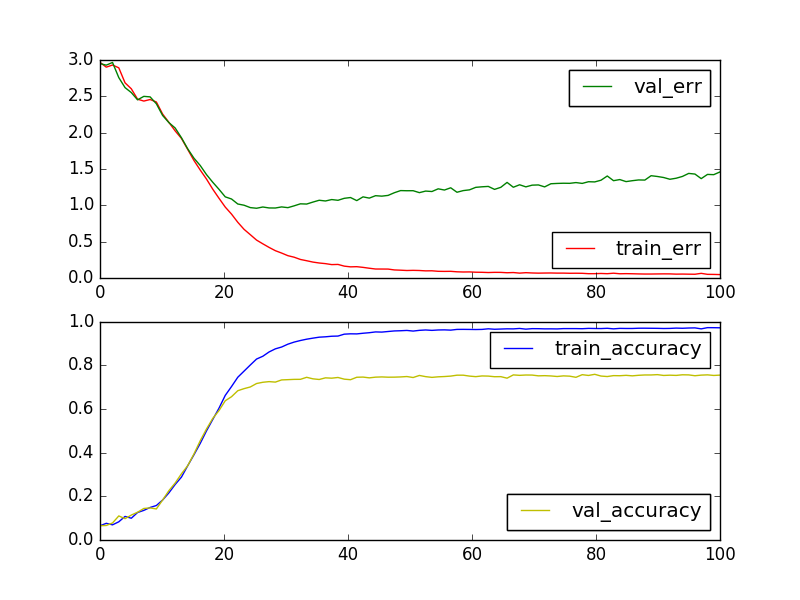
\includegraphics[height=1.6in]{../text/text_classification/figures/lstm_glove_noconv.png}
        \caption
            {\scriptsize LSTM with GloVe embeddings and no convoluion layer}
    \end{subfigure}%
    ~ 
    \begin{subfigure}[b]{0.48\textwidth}
        \centering
        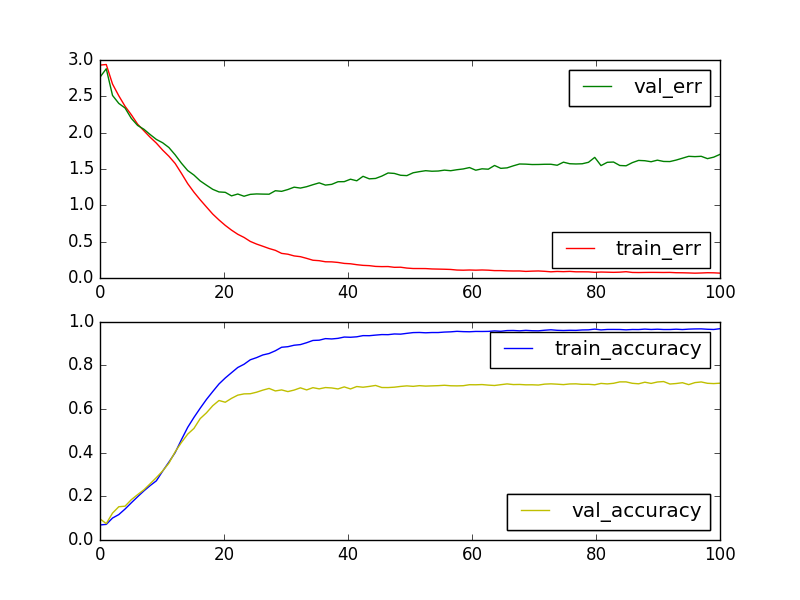
\includegraphics[height=1.6in]{../text/text_classification/figures/lstm_glove_conv.png}
        \caption
            {{\scriptsize LSTM with GloVe embeddings and convoluion layer}} 
    \end{subfigure}
    \vskip\baselineskip
    \begin{subfigure}[b]{0.48\textwidth}
        \centering
        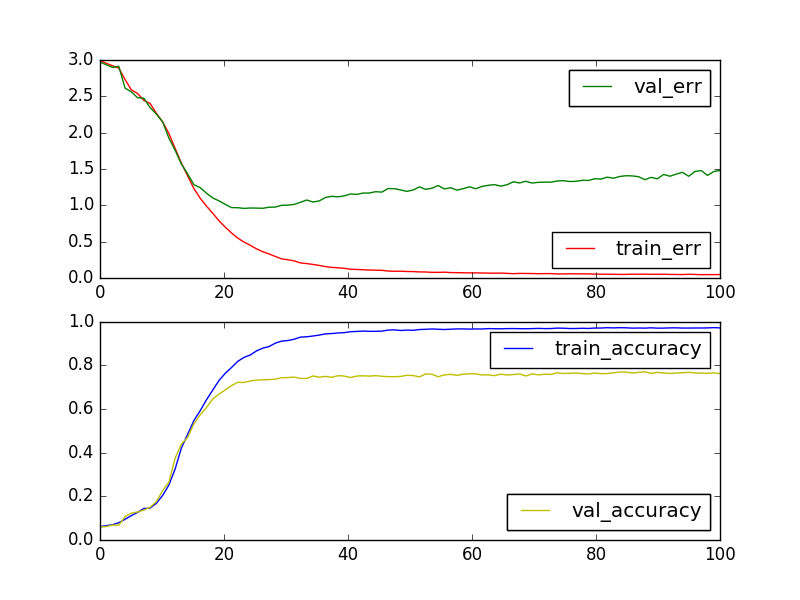
\includegraphics[height=1.6in]{../text/text_classification/figures/lstm_w2v_noconv.png}
        \caption[Network2]%
            {{\scriptsize LSTM with Word2vec embeddings and no convoluion layer}} 
    \end{subfigure}%
    ~ 
    \begin{subfigure}[b]{0.48\textwidth}
        \centering
        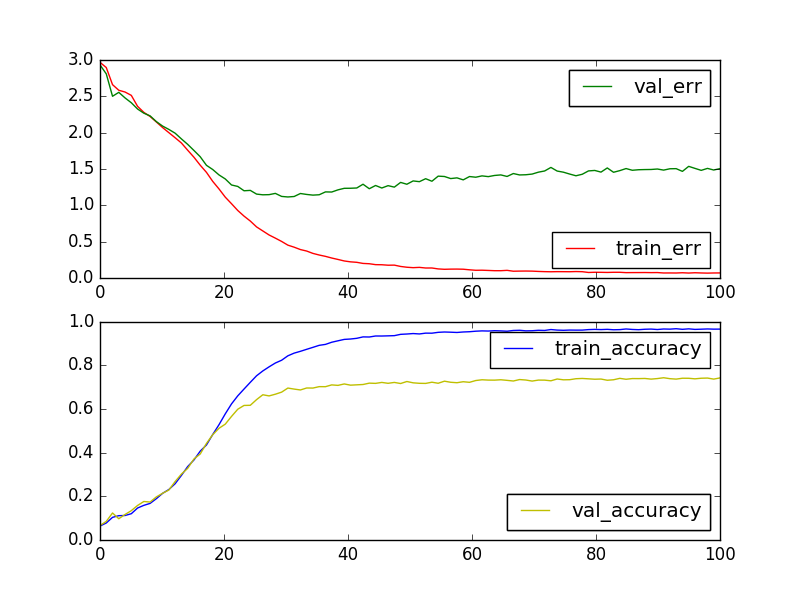
\includegraphics[height=1.6in]{../text/text_classification/figures/lstm_w2v_conv.png}
        \caption[Network2]%
            {{\scriptsize LSTM with Word2vec embeddings and convoluion layer}} 
    \end{subfigure}
    \vskip\baselineskip
    \centering
    \begin{subfigure}[b]{0.48\textwidth}
        \centering
        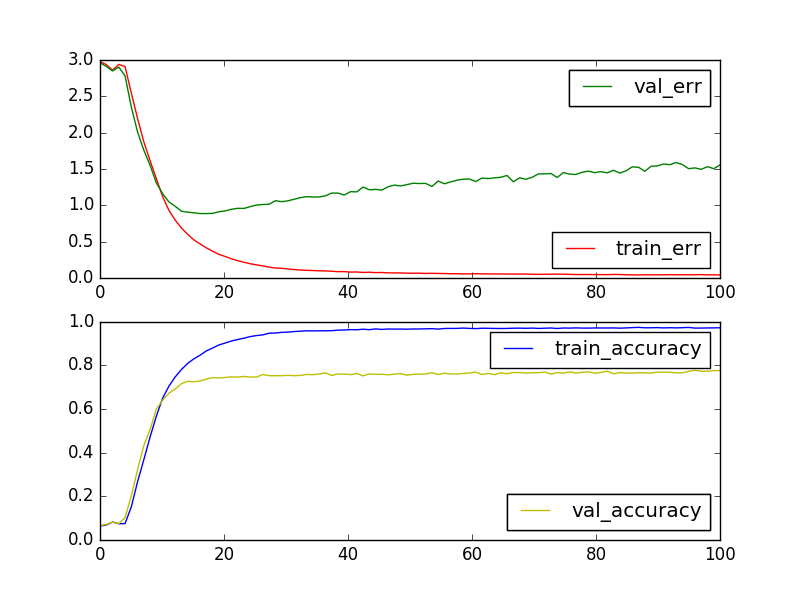
\includegraphics[height=1.6in]{../text/text_classification/figures/gru_glove_noconv.png}
        \caption[Network2]%
            {{\scriptsize GRU with GloVe embeddings and no convoluion layer}} 
    \end{subfigure}%
    ~ 
    \begin{subfigure}[b]{0.48\textwidth}
        \centering
        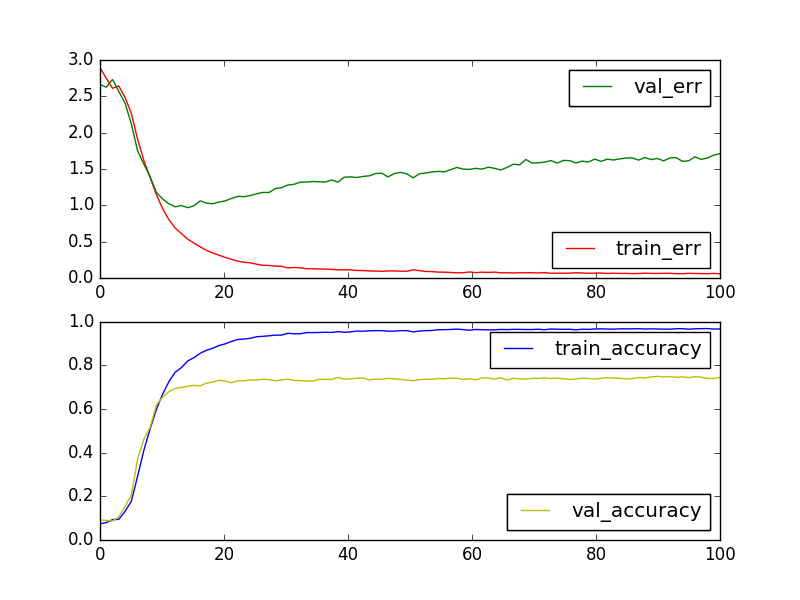
\includegraphics[height=1.6in]{../text/text_classification/figures/gru_glove_conv.png}
        \caption[Network2]%
            {{\scriptsize GRU with GloVe embeddings and convoluion layer}} 
    \end{subfigure}
    \vskip\baselineskip
    \begin{subfigure}[b]{0.48\textwidth}
        \centering
        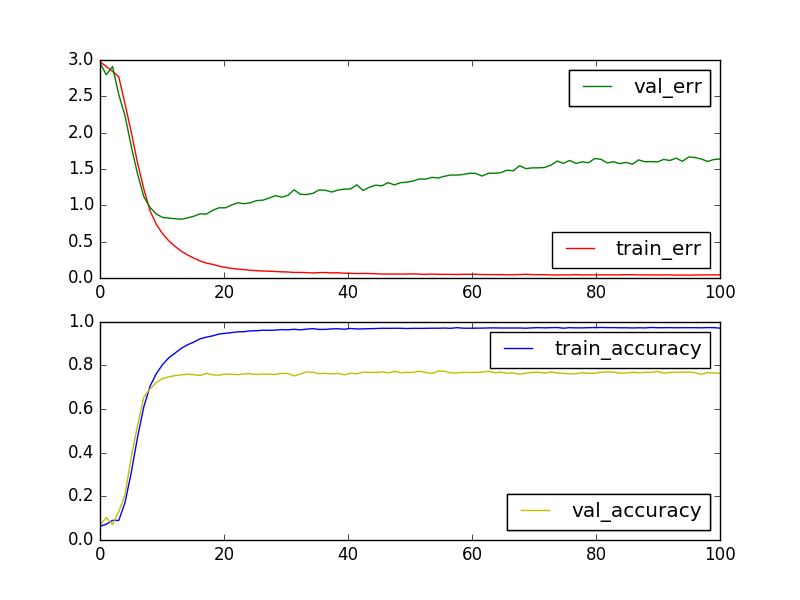
\includegraphics[height=1.6in]{../text/text_classification/figures/gru_w2v_noconv.png}
        \caption[Network2]%
            {{\scriptsize GRU with Word2vec embeddings and no convoluion layer}} 
    \end{subfigure}%
    ~ 
    \begin{subfigure}[b]{0.48\textwidth}
        \centering
        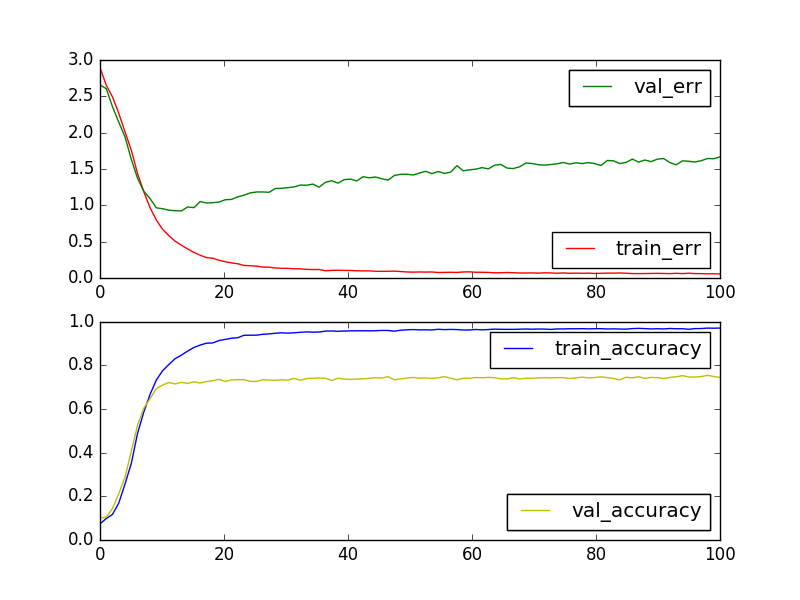
\includegraphics[height=1.6in]{../text/text_classification/figures/gru_w2v_conv.png}
        \caption[Network2]%
            {{\scriptsize GRU with Word2vec embeddings and convoluion layer}} 
    \end{subfigure}
    \caption{\small Convergence Performance for different RNN settings}
    \label{Fig1}
\end{figure}





% \section{Revised Plan}
% During preliminary experiments, we have tried classic approaches such as SVM and neural network methods such as CNN based on different word representations. We did a basic research on Recurrent Neural Networks methods and found many of them required a long computing and training time. For future plans:
% \begin{itemize}
% \item We will continue investigating RNN approaches like (LSTM and GRU) that could train and validate within reasonable amount of time.
% \item We will continue learning and experimenting with other variants of CNN and RNN approaches.
% \item We will compare all these classical and more advanced and complex approaches based on classification accuracy and training time. Analyze the reason behind the results and trade-offs among different approaches.
% \end{itemize}

\section{Discussion and Analysis}
\subsection{SVM}
According to our results, SVM’s performance is highly unstable across different hyper-parameter settings.  For example, C is a regularization parameter that controls the trade off between the achieving a low training error and a low testing error that is the ability to generalize your classifier to unseen data. Different C’s result in very different classification performance: 87\% when C=1 and 55\% when C=0.1 with linear kernel tested on 20 Newsgroups dataset.  Also, different kernels will also result in very different accuracy results. For example, linear kernel achieves 55\% but polynomial kernel only achieves 5\% accuracy when C=0.1 tested on 20 Newsgroups dataset.

Recognizing that SVM is a less computationally complex algorithm than the Artificial Neural Networks, we conclude that SVM is preferable at least for many short text documents in a relatively few well populated categories. Furthermore, SVM depends on feature construction with many sophisticated techniques such as TF-IDF, etc. It requires more consideration and effort on feature engineering and extraction than CNN or RNN and performs less stable with different hyper-parameters and extracted features.


\subsection{CNN}
In summary, we find that the best CNN’s classification accuracy is on par with the best RNN result as well as SVM accuracy. However, CNN shows instability in performance with different classification task. In specific, with the same CNN model, it performs better and more stable with classification problem with fewer categories. In terms of, convergence performance and training time, CNN offers the most competitive performance, with faster convergence rate and less training time. This is mainly due to the parameter sharing in CNN, which accelerate training by reducing the number of parameters to train.


\subsection{RNN}
For using RNNs to perform classification, we have run experiment on both LSTMs and GRUs. The same as the case of CNN, we have tried 2 different kinds of word embeddings. Finally, to reduce the number of parameters trained and accelerate the training, we added convolution layer before a LSTM or GRU. Therefore, we have obtained in total 8 sets of results.

As can be seen from the results, the 4 results for GRU have higher accuracy than those obtained by using LSTM. Although the difference is not significant, with the largest gap of 2.67\%, the GRU group could be faster than the LSTM group by up to  23\%. This proves that GRU is potentially more suitable for text classification task.  In addition, in terms of convergence performance, GRU converges using much less number epochs than LSTM, as shown in 5.3. This is due to GRU has less complex structure and fewer trainable parameters then LSTM.

The convolution layer added before the RNN layer can reduce the training time to almost half the time taken without the convolution layer. Although there are some degradation in the accuracy, it was kept within 3\% for the GRU case. Notice that  in our setup the convolution layer was not fine tuned to maximize the accuracy due to the limitation of the project time line. Therefore, we believe that with some hyper-parameter tuning, adding convolution layer before RNN cloud potentially obtain the same classification accuracy with much lower training time.

Finally, comparing different word embeddings, we can see that the results are very close to each other with Word2vec embedding has higher accuracy for the LSTM group, but lower accuracy for the GRU group. In terms of training speed the two kind of word embeddings shows no significant difference. From this result we can see that both word embeddings are suitable for text classification, and there's no evidence that one is superior than the other.




\section{Conclusion and Future Work}
In this paper, we study the text classification problem using different deep learning approaches.  We compare and analyze the performance of different text classification approaches, such as Support Vector Machine (SVM), Convolutional Neural Network (CNN) and Recurrent Neural Network (RNN), etc. We find that SVM combined with feature engineering provides fairly competitive accuracy. The best CNN and RNN results are similar to SVM results. As for RNN, GRU performs on par with LSTM, but with better convergence properties. We also propose and implement a method to reduce the training time for RNN training with only a small fraction of accuracy loss.

For future work, we plan to tackle the same problem with more complex models. We plan to use much deeper models for both CNN and RNN. In addition, we plan to leverage variants of more advanced language models such as character-level CCN [1] and Recurrent Convolutional Neural Networks [2], etc. We expect to get better classification accuracy from these complex models.

\section*{References}

\small

[1] Zhang, X., Zhao, J., \& LeCun, Y. (2015). Character-level convolutional networks for text classification. In Advances in neural information processing systems (pp. 649-657).

[2] Lai, S., Xu, L., Liu, K., \& Zhao, J. (2015, January). Recurrent Convolutional Neural Networks for Text Classification. In AAAI (Vol. 333, pp. 2267-2273).

[3] Yin, W., Kann, K., Yu, M., \& Schütze, H. (2017). Comparative Study of CNN and RNN for Natural Language Processing. arXiv preprint arXiv:1702.01923.

[4] Wang, S., \& Manning, C. D. (2012, July). Baselines and bigrams: Simple, good sentiment and topic classification. In Proceedings of the 50th Annual Meeting of the Association for Computational Linguistics: Short Papers-Volume 2 (pp. 90-94). Association for Computational Linguistics. Chicago.

[5] Bishop, C. M. (2006). Pattern recognition and machine learning. springer. Chicago.

[6] Kim, Y. (2014). Convolutional neural networks for sentence classification. arXiv preprint arXiv:1408.5882.

[7] Mikolov, T., Chen, K., Corrado, G., \& Dean, J. (2013). Efficient estimation of word representations in vector space. arXiv preprint arXiv:1301.3781.

[8] Pennington, J., Socher, R., \& Manning, C. (2014). Glove: Global vectors for word representation. In Proceedings of the 2014 conference on empirical methods in natural language processing (EMNLP) (pp. 1532-1543).

[9] Cho, K., Van Merriënboer, B., Gulcehre, C., Bahdanau, D., Bougares, F., Schwenk, H., \& Bengio, Y. (2014). Learning phrase representations using RNN encoder-decoder for statistical machine translation. arXiv preprint arXiv:1406.1078.

[10] Chung, J., Gulcehre, C., Cho, K., \& Bengio, Y. (2014). Empirical evaluation of gated recurrent neural networks on sequence modeling. arXiv preprint arXiv:1412.3555.

[11] Word2vec embeddings. http://www.cs.toronto.edu/~guerzhoy/411/proj3/embeddings.npz

[12] Lee, J. Y., \& Dernoncourt, F. (2016). Sequential short-text classification with recurrent and convolutional neural networks. arXiv preprint arXiv:1603.03827.

[13] Yin, W., Kann, K., Yu, M., \& Schütze, H. (2017). Comparative Study of CNN and RNN for Natural Language Processing. arXiv preprint arXiv:1702.01923.

[14] Conneau, A., Schwenk, H., Barrault, L., \& Lecun, Y. (2017). Very deep convolutional networks for text classification. In Proceedings of the 15th Conference of the European Chapter of the Association for Computational Linguistics: Volume 1, Long Papers (Vol. 1, pp. 1107-1116).



\end{document}
